% Introduction
% ------------

\section{Introduction}

Sustainable software engineering has become an active area of
research~\cite{2012:penzenstadler}.
Sustainable software is expected to remain available in new platforms in the
future continually meeting new environmental needs employing adequate evolution
in the face of ever-changing conditions~\cite{allen2017engineering}.
%
Software sustainability is often related to
the fulfillment of non-functional requirements and 
the quality of the software~\cite{2014:penzenstadler,2016:hthesis}.
It comprises 4+1 dimensions:    
\citeauthor{2002:goodland}'s dimensions for sustainability analysis -- human,
social, economic and environmental~\cite{2002:goodland}, and the technical
dimension proposed by~\citet{2013:penzenstadler}.
%
Technical sustainability is concerned with the long-term usage of software and
its capacity to evolve with changing conditions and
requirements~\cite{2012:penzenstadler,2013:penzenstadler}.

Academic software is a software developed to collect, process, or analyze research results published in the academic literature, mostly written by researchers that needed to use this kind of software~\cite{allen2017engineering}. We included in the set of academic software projects studied in this work any software listed by the authors among the outputs of a publication, publicly available, identified by its authors with URLs for download, from the domain of static analysis.
%
For academic software technical sustainability applies: to be sustainable, academic software must be maintained, improved and released for others’ use. However, a research work itself requires visibility, reliability, and reproducibility. Therefore, academic software must address these crucial requirements for science. 

\begin{figure}[htb]
  \centering
  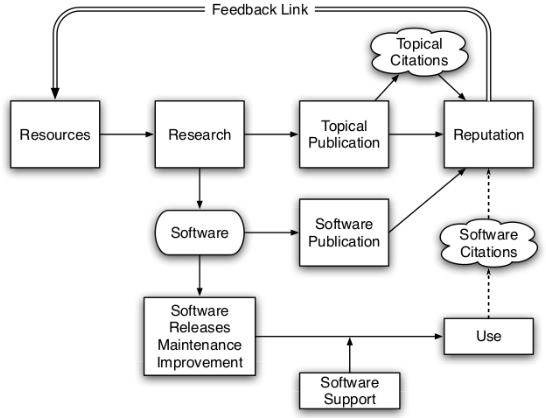
\includegraphics[scale=0.4]{figs/scientific-reputation-diagram.png}
  \caption{A depiction of the reputation incentives in a mixed science and academic software practice (from \cite{howison2011scientific}).}
  \label{scientific-reputation-diagram}
\end{figure}

Figure~\ref{scientific-reputation-diagram} presents a depiction of a mixed
science and academic software practice scenario \cite{howison2011scientific}.
%
Academic software is part of a scientific ecosystem that is concerned with
research and reputation~\cite{howison2011scientific}.  Research may generate
\textit{topical publications} that address a research question and receive
\textit{topical citations}
that contribute to increasing academic
reputation~\cite{howison2011scientific,howison2015understanding}.  
Research may also produce academic software or
generate related \textit{software publications}
describing the software produced in the course of
research~\cite{howison2015understanding}. These software publications and
the academic software, but mostly the latter, receive \textit{software citations}
that may also contribute to increasing academic reputation.
%
Moreover, researchers should share their source code and other artifacts
required for visible, reliable, and reproducible science. Otherwise, the lack of
visibility of academic software can make replication and reliability assessment
unfeasible, generate rework, and inefficiently consume the limited resources of
science.

In this context, new aspects and strategies deserve to be investigated as possible
indicators for the sustainability of academic software. They should be
analyzed together with standard technical concerns. In this paper, we
investigate three candidates: software publicization, evolution stage, and
software recognition.

The publicization of academic software is related to making it available
explicitly from a given URL in a publication regarding the software.
Publicization may deal with opening the development of the software so that
other developers can access the code -- under a license~\cite{SSI,SSI:2013}.
Outside developers with access to source code can adapt the academic software
to meet their exact needs, while the community can give back to the project any
fixed bugs or new functionality.  This approach can increase the number of
citations to software and software publications, increasing academic
reputation.

The evolution stage of the academic software can be an indicator of its
technical sustainability.  The staged model for the software life cycle
\cite{rajlich2000staged} provides a useful and straightforward model from the
perspective of developers/scientists and end-users to understand the academic
software as well as its stage of evolution (initial development, evolution,
servicing, phase-out, or close-down).  Such information may be useful to
support decision-making on adopting academic software for use or even as a
target for contribution. 

Finally, software recognition can be used as an external indicator 
for academic software sustainability -- although
unfortunately, the level of recognition and reward for the
academic software and those who review or develop it,
is not proportional to the software importance \cite{goble2014better}.  
The recognition of academic software can be assessed based 
on ``mentions'' to different kinds of ``uses'' 
in the scientific literature, 
including contributions to the software. 

\myparagraph{Research Strategy}
We conducted three exploratory studies to investigate the sustainability of
academic software for static analysis, a field with tradition
in the development of tools to support research in different areas of
computer science.
We selected software publications on static analysis tools
from \textit{ASE (Automated Software Engineering)}  and
\textit{SCAM (Working Conference on Source Code Analysis \& Manipulation)}.

We chose these two conferences based on the principle of being traditional Software Engineering conferences, having recognized studies on software analysis and, thus, increasing the number of academic software of static analysis found among its publications.

% STUDY 1
The first study investigated the publicization of academic software.
We performed
a ``systematized'' literature review \cite{2009:grant}
and identified \SoftwareCount \ static analysis software tools
published in articles at ASE and SCAM.
Thereby, we characterized them concerning availability for download,
source code access, distribution form, and license.

% STUDY 2
The second study investigated the life cycle of academic software. We
characterized academic software (with online presence,
selected from the first study)
with respect to their evolution stage,
based on releases, versions, and the
number of modules for each software version with source code available.

% STUDY 3
The third study investigated the recognition of academic software. This study
took the set of \SoftwareCount \ academic software identified in the first
study as its starting point. A second literature review performed on the ACM
and IEEE digital libraries found \SearchUniqueCount \ publications that have
``mentions'' of the following types to the set of academic software:
Citations, Uses, and Contributes.

%The paper is organized as follows.
In summary, in thist paper, we present the exploratory studies on publicization
(Section~\ref{study1}), software lifecycle (Section~\ref{study3}), and
recognition (Section~\ref{study2}), as well as, provide a discussion on them
(Section~\ref{sec:discussion}).  Section~\ref{sec:conclusions} presents final
remarks about the studies.
